
\documentclass[a4paper, oneside, 11pt]{report}
\usepackage{epsfig,pifont,float,multirow,amsmath,amssymb}
\newcommand{\mc}{\multicolumn{1}{c|}}
\newcommand{\mb}{\mathbf}
\newcommand{\mi}{\mathit}
\newcommand{\oa}{\overrightarrow}
\newcommand{\bs}{\boldsymbol}
\newcommand{\ra}{\rightarrow}
\newcommand{\la}{\leftarrow}
\usepackage{algorithm}
\usepackage{algorithmic}
\topmargin = 0pt
\voffset = -80pt
\oddsidemargin = 15pt
\textwidth = 425pt
\textheight = 750pt

\begin{document}

\begin{titlepage}
\begin{center}
\rule{12cm}{1mm} \\
\vspace{1cm}
{\large  CMP-6048A Advanced Programming}
\vspace{7.5cm}
\\{\Large Project Report - 10 January 2024}
\vspace{1.5cm}
\\{\LARGE MATBAP: Maths Interpreter software}
\vspace{1.0cm}
\\{\Large Group members: \\ Igor Stepanenko, Lyra, Liam Farese\ }
\vspace{10.0cm}
\\{\large School of Computing Sciences, University of East Anglia}
\\ \rule{12cm}{0.5mm}
\\ \hspace{8.5cm} {\large Version 2.0}
\end{center}
\end{titlepage}


\setcounter{page}{1}
%\pagenumbering{roman}
%\newpage


\begin{abstract}
Please replace this section with your own abstract. An abstract is a brief summary (maximum 250 words) of your entire project. It should cover your objectives, your methodologies used, a brief developmental history, your final results, in particular covering the optional tasks, and a discussion and conclusion. You do not cover the literature or background in an abstract nor should you use abbreviations or acronyms. The remainder of this report template has clear chapter titles and we suggest to stick to these although you can organise your material inside each chapter to your own preferences. A guideline in size is approximately 3,500 words (not including abstract, captions and references) but no real limit on figures, tables, diagrams, pseudo-code etc.
\end{abstract}

\chapter{Introduction}
\label{chap:intro}

\section{Project statement}
This project will be a Maths Interpreter software with extensions aiming
towards a Turing complete language. It will be used to evaluate expressions, define
variables and functions, and plot functions of two variables. The software
will allow the user to enter expressions and equations using a custom language which is processed by a lexer, parser and evaluator. Plots of mathematical equations will be interactive. Additional functionality might include root finding, differentiation and integration. The software will be developed keeping in mind software engineering principles such as low coupling and high cohesion achieved through Model-View-ViewModel and Inversion of Control patterns. 

\section{Aims and objectives}
The main aim is to develop Matbap, a maths interpreter software for solving and plotting mathematical expressions. Main objectives include:
\begin{itemize}
    \item Create Lexer, Parser and Evaluator in F\# to process mathematical expressions and equations to plot.
    \item Develop a Graphical User Interface (GUI) in C\# for user interaction.
    \item Integrate F\# and C\# components keeping in mind low coupling.
\end{itemize}

\noindent % Start a new paragraph without indentation
They are broken further into subtasks in this MoSCoW table \ref{appendix:moscow} 


\chapter{Background}
The development of maths software capable of plotting graphs has become significantly easier in recent years, because of integration of technology in education and research. Therefore, it is important we acknowledge key software and literature in this field.

Desmos\cite{Desmos:2023} software offers a graphical calculator that changed the way students learn mathematics by providing an intuitive UI and robust plotting functionality to allow for visualisations of complex functions and equations.

MATLAB\cite{Matlab:2023} is the mainstream tool in the field of mathematical computing, visualising and programming. It offers extensive tooling that includes signal and image processing, which is why it is widely used in academia and industry.

The Windows Presentation Foundation (WPF)\cite{WPF:2023} documentation provided by Microsoft Learn offered tutorials and guidance on creating desktop user interfaces. WPF’s powerful data-bindings were critical in displaying mathematical data back to the user.

The Dependency Injection (DI) \cite{DI:2023} documentation from Microsoft Learn described the design pattern that produces more testable and modular software. In the context of our application, this pattern allowed for dynamic integration of different services like equation evaluator and plotting evaluator, and as a result made our software more maintainable and scalable.

The Model-View-ViewModel (MVVM)\cite{MVVM:2022} documentation from Microsoft Learn describes the architecture, which is primarily used with WPF applications due to its powerful data-binding features. MVVM creates a clear separation of concerns where business logic is decoupled from the UI. This architecture was important in developing our software because it allowed for maintainable and scalable code, which could handle mathematical calculations and user interactions.


\chapter{Development History}\label{Chap:DevHist}

\section{Sprint 0: Setup development infrastructure}
At the very start of this project, we needed to setup and integrate essentials tools that have been critical in streamlining workflow and improving teamwork.

\subsection{Jira Board}
To track our work, we chose Jira\cite{Atlassian:JIRA} - tool for task management and sprint planning, which provided us with visual representation of our project's progress. We setup a Jira Board(link \ref{ap-jira-link}) that helped us create a backlog tickets, that can be assigned to a team member and tracked in To Do, In Progress and Done columns.

\subsection{Visual Studio Project}
Next we configured a Visual Studio solution that could reference a F\# application in a C\# application as a DLL\cite{DLL}.

\subsection{GitHub repository}
We setup a version a control system for our codebase - GitHub repository(link - \ref{github-repo}). This enabled us to collaborate, peer review each others work and keep a history of contributions to the project. A significant objective was to setup a Continuous Integration (CI)\cite{Atlassian:CI} using GitHub Actions\cite{GitHubDocs:Actions} to ensure that our codebase remains bug free through automated testing before any changes are merged to the main branch.

\subsection{Conclusion}
This sprint has laid foundation to our development journey. Setting up tools like Jira, GitHub and Visual Studio not only streamlined our workflow but also enabled us to be an effective and efficient team.

% https://liamfarese.atlassian.net/browse/AP-8
\section{Sprint 1: Basic arithmetic calculations, Basic GUI.}
In our first sprint, we focused on building the foundation of our maths interpreter, like basic arithmetic calculations and basic GUI. Our objective was to develop a software that mathces the spec requirements and is a robust and scalable application, keeping in mind maintainability and testability.

\subsection{Lexer}
We developed a lexer that would tokenise expressions consisting of digits, binary operations, identifiers and functions like sin, cos and tan. One of the challenges we faced was unfamiliarity with F\# and functional programming, especially the recursive nature of this programming paradigm. 

\subsection{Parser}
We developed a parser that would parse and evaluate expressions that followed this basic grammar.
\begin{verbatim}
 <E>    ::= <T> <Eopt>
 <Eopt> ::= + <T> <Eopt> | - <T> <Eopt> | <empty>
 <T>    ::= <NR> <Topt>
 <Topt> ::= * <NR> <Topt> | / <NR> <Topt> | <empty>
 <NR>   ::= <int> | <float> | (E)
\end{verbatim}

\subsection{Basic GUI}
We used WPF\cite{WPF:2023} with C\# to develop a basic GUI, focusing on maintainability, testability, and scalability. App's architecture consists of several design patterns like Model-View-ViewModel\cite{MVVM:2022}, that improves GUI's responsiveness to user interactions and Dependency Injection\cite{DI:2023} for better modularity and easy maintenance. The GUI was a minimalistic interface allowing users to enter expressions and view the answers - see Figure \ref{basicgui}.

\subsection{Testing}
Thorough unit tests were written for both the C\# app and the F\# engine. Table \ref{sprint1-lexer-test} includes unit test for the Lexer. Table \ref{sprint1-parser-test} includes unit tests for the Parser. The table with GUI unit tests can be seen in \ref{sprint1-gui-test}. The use of the MVVM and Dependency Injection patterns allowed us to to use the Moq\cite{Moq} mocking library to mock Model behaviours in our ViewModel. This allowed us to test code in isolation without relying on behaviour of real dependencies and to have control over what is returned from the mocked methods. As a result our code coverage was above 80\%.

\subsection{Conclusion}
The first sprint laid a solid foundation for our maths interpreter. The lexer and parser were capable of evaluation basic arithmetic expressions and the GUI was providing simple interface for user interaction. Our testing strategy set a ensured that future features were build upon a reliable codebase. 

%https://liamfarese.atlassian.net/browse/AP-30
\section{Sprint 2: Modulo and Power, Correct treatment of integers and floats, Help Menu, Lexer error handling, Link C\# app with F\# engine}

In our second sprint, we focused on improving functionality and user experience of our maths interpreter. Key improvements were support for modulo and power operators, correct handling of integers and floats, better errors in the Lexer and linking our GUI with the interpreter.

\subsection{Lexer}
We updated our lexer with better errors. Now it returns error messages that include the problematic token and its position. This improvement helped us in our debugging processes and provided more clarity to users.

\subsection{Parser}
After a review from the teaching team, we identified a bug. We didn't correctly handle our floats and integers. Previously, integers were cast to floats in order to allow calculation with them. Our fix allowed integers and floats to be handled separately: integer operations would always return integers and the same would happen for floats. The updated BNF reflects this change:
\begin{verbatim}
<E>    ::= <T> <Eopt>
<Eopt> ::= + <T> <Eopt> | - <T> <Eopt> | <empty>
<T>    ::= <NR> <Topt>
<Topt> ::= * <NR> <Topt> | / <NR> <Topt> | <empty>
<NR>   ::= <num> | (E)
<num>  ::= <int> | <float>
\end{verbatim}

Furthermore, we added support for modulo (\%) and power (\textasciicircum) operators. This is reflected in this updated BNF:
\begin{verbatim}
<E>    ::= <T> <Eopt>
<Eopt> ::= + <T> <Eopt> | - <T> <Eopt> | <empty>
<T>    ::= <P> <Topt>
<Topt> ::= * <P> <Topt> | / <P> <Topt> | % <P> <Topt> | <empty>
<P>    ::= <NR> <Popt>
<Popt> ::= ^ <NR> <Popt> | <empty>
<NR>   ::= <num> | (E)
<num>  ::= <int> | <float>
\end{verbatim}


\subsection{Updated GUI}
The GUI was updated with a Help window, that showed all supported tokens. This addition improved user accessibility. The connection of our GUI to our interpreter allowed for real time calculations. The screenshot of updated GUI can be seen in TODO \ref{helpgui}.

\subsection{Testing}
We updated our unit tests to validate new features and fixed bugs. They can be seen under TODO\ref{}

\subsection{Conclusion}
Sprint 2 has made good progress in developing our maths interpreter. The introduction of new operators and the correction of behaviour around integer and floats improved our app's versatility and better matched requirements. The lexer's errors and updated GUI improved user experience.


% https://liamfarese.atlassian.net/browse/AP-42
\section{Sprint 3: Unary minus, Assign variables, Plotting lines and polynomials}
% https://liamfarese.atlassian.net/browse/AP-50
\section{Sprint 4: AST Parser and AST Evaluator}
\section{Sprint 5: Differentiation, Adding tangents, Multiple Plots}
\section{Sprint 6: Visualise AST}
\section{Sprint 7: Root finding}
\section{Sprint n: And whatever we complete before we submit this}



\chapter{Final deliverable}\label{Impl}

In this chapter you cover the final or ``ultimate'' version of your project. It will show the final BNF, the final GUI, the architecture (which should be MVVM or MVC) that includes UML diagrams, additional algorithms if not already included in the previous sprint sections.

\section{Final BNF}

\section{Final GUI}

\section{Code architecture}

\section{Algorithms}

Algorithms can be described in this chapter if not already covered in previous sections. Pseudo-code is preferred over code snippets. If you use the latter then make sure it is well commented inside the code or via the figure caption. 

\begin{algorithm}[th]
\caption{ The Newton-Raphson method }
\begin{algorithmic}[1]
\STATE Initialise root based on estimate
\STATE Set stop criterion
\\ \texttt{const double error = 0.000001;}
\WHILE {stop criterion not met}
	\STATE Compute f(root)
	\STATE Compute f'(root)
	\STATE root := root - f(root)/f'(root)
\ENDWHILE
\end{algorithmic}
\end{algorithm}


Note that code snippets or lists of crucial programming code or large UML diagrams should go in Appendix \ref{app:other} (or further appendices).

\subsection{Testing}

Describe what testing you have done on the interpreter (lexer, parser and execution), GUI and GUI-Interpreter communication, plotting, etc. Table \ref{Table2} in Appendix \ref{app:test} should be completed to do basic arithmetic expression tests.


\chapter{Discussion, conclusion and future work}

Briefly discuss  your achievements and put them in perspective with the MoSCoW analysis you specified in Table \ref{Table1}. Also discuss future developments and how you see the deliverable improving if more time could be spent. Note that this section should not be used as a medium to vent frustrations on whatever did not work out (group issues, not enough time, illness, etc.) as this should be dealt with separately - keep it professional!


\bibliographystyle{apalike}
\raggedright
\bibliography{References}


\appendix
\chapter{Contributions}

State here the \% contribution to the project of each individual member of the group and describe in brief what each member has done (if this corresponds to particular sections in the report then please specify these).

\chapter{Aims and objectives}
\section{MoSCoW table}
\label{appendix:moscow}
\begin{table}[h]
\caption{MoSCoW}
\begin{center}
\begin{tabular}{|p{1in}|p{2in}|p{2.5in}|} \hline
Priority & Task & Comments \\ \hline \hline
\multirow{3}{1in}{Must}
& Solve arithmetic expressions & Works with ints and floats, processing is left-associative, BODMAS/BIDMAS rules apply \\ \cline{2-3}
& Have basic GUI & Input textbox, output textbox and help functionality \\ \cline{2-3}
& Have variable assignment & Assignment token, Grammar change, Stored in a symbol table \\ \cline{2-3}
& Be tested & Unit and functionally tested \\ \cline{2-3}
& Have basic plotting & Plotting area in GUI window to visualise mathematical functions: lines and polynomials \\ \hline \hline
\multirow{3}{1in}{Should}
& AST Parser & Parser constructs an Abstract Syntax Tree \\ \cline{2-3}
& Functions & Works with built-in functions such as cos, sin, tan, exp, log  \\ \cline{2-3}
& Multiple plots & User can plot multiple equations and clear the plotting area \\ \hline \hline
\multirow{3}{1in}{Could}
& For loops & \\ \cline{2-3}
& Conditionals & If statements \\ \cline{2-3}
& Rational numbers & \\ \cline{2-3}
& Complex numbers & \\ \cline{2-3}
& Rational equations plotting & Plot equations like 1/x that produce more than 1 line \\ \hline \hline
\multirow{3}{1in}{Will not}
& Compiler & Too much work to implement a compiler in a given timeframe \\ \cline{2-3}
& Static typing & Making our language statically typed requires a very strong typing system in place which is too hard to implement in a give timeframe \\ \hline
\end{tabular}
\label{Table1}
\end{center}
\end{table}

\chapter{Testing}
\label{app:test}

\section{F\# engine unit testing}

\begin{table}[h]
\caption{Sprint 1, Lexer unit tests}
\label{sprint1-lexer-test}
\begin{tabular}{|l|l|l|}
\hline
\textbf{Expression}        & \textbf{Pass/Fail} & \textbf{Comment}                      \\ \hline
1a+12                      & Pass               & Tokenises variable, int and operation \\ \hline
33.3/(12 + 3.5a)           & Pass               & Float/Int distinct tokenisation       \\ \hline
sin(43)/cos(1.5) * tan(34) & Pass               & Function tokenisation                 \\ \hline
4 \% 2                     & Pass               & Modulus tokenisation                  \\ \hline
4\textasciicircum{}3       & Pass               & Power tokenisation                    \\ \hline
1. + 43                    & Pass               & Lexer error                           \\ \hline
1.4.2                      & Pass               & Lexer error                           \\ \hline
1\&                        & Pass               & Lexer error                           \\ \hline
\end{tabular}
\end{table}

\begin{table}[h]
\caption{Sprint 1, Parser unit tests}
\label{sprint1-parser-test}
\begin{tabular}{|l|l|l|}
\hline
\textbf{Expression} & \textbf{Pass/Fail} & \textbf{Comment}                                                                     \\ \hline
2+10                & Pass               & Parses and evaluates basic addition                                                  \\ \hline
7-3                 & Pass               & Parses and evaluates basic subtraction                                               \\ \hline
5*7                 & Pass               & \begin{tabular}[c]{@{}l@{}}Parses and evaluates basic \\ multiplication\end{tabular} \\ \hline
12/8                & Pass               & \begin{tabular}[c]{@{}l@{}}Parses and evaluates basic \\ division\end{tabular}       \\ \hline
5*2.3               & Pass               & Parses and evaluates integers with floats                                            \\ \hline
13.56-6+14*20.1     & Pass               & Order of operations                                                                  \\ \hline
5-2.5/(6.0+6.5)+1   & Pass               & Order of operations using brackets                                                   \\ \hline
1\&                 & Pass               & Operators without an operand between                                                 \\ \hline
6+-2                & Pass               & Operators without an operand between                                                 \\ \hline
5/                  & Pass               & Operator without an operand following                                                \\ \hline
*                   & Pass               & Operator with no operands at all                                                     \\ \hline
(()                 & Pass               & Opening a bracket without closing it                                                 \\ \hline
())                 & Pass               & Closing a bracket without having opened a matching one                               \\ \hline
1/0                 & Pass               & Division by 0                                                                        \\ \hline
\end{tabular}
\end{table}



\newpage
\section{C\# GUI unit testing}

\begin{table}[h]
\caption{Sprint 1, GUI unit test}
\label{sprint1-gui-test}
\begin{tabular}{|l|l|l|}
\hline
\textbf{Input} & \textbf{Pass/Fail} & \textbf{Comment}                 \\ \hline
123            & Pass               & Updates the View with user input \\ \hline
\end{tabular}
\end{table}


\section{Plot testing}

\chapter{GUI}
\label{app:gui}
\section{Basic GUI}
\begin{figure}[H]
\begin{center}
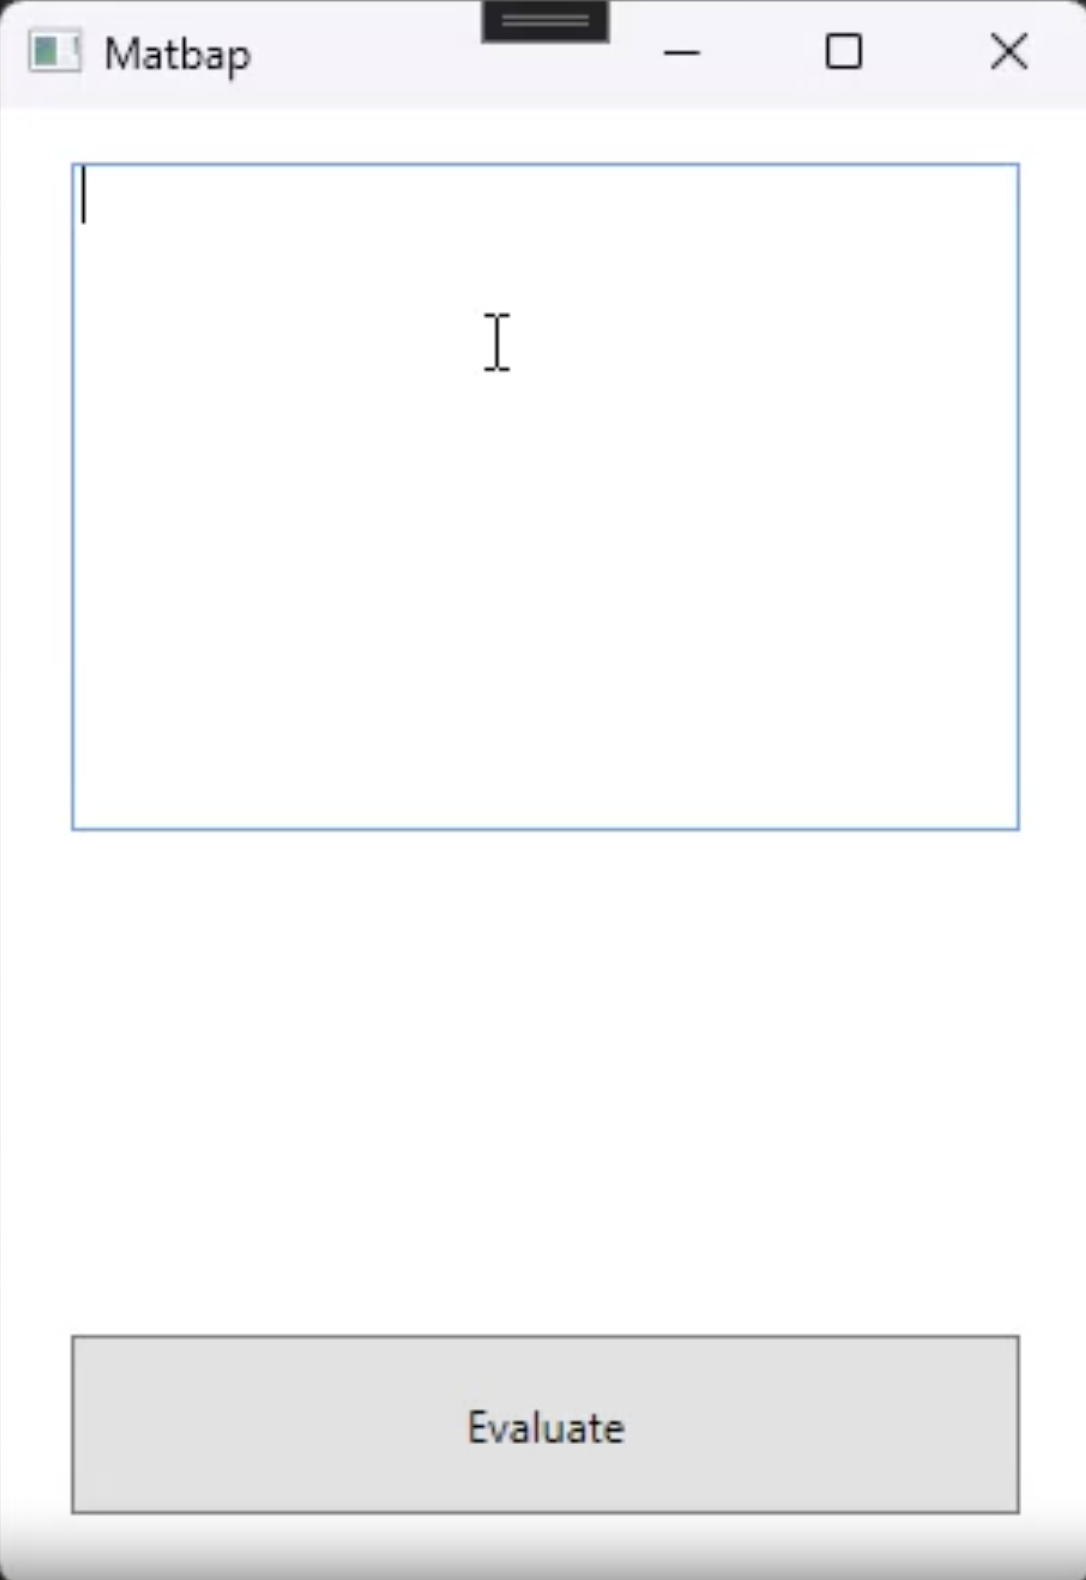
\includegraphics[scale=0.3 ]{Basic GUI.png}
\caption{Our first basic GUI}
\label{basicgui}
\end{center}
\end{figure}

\section{Updated GUI with Help Window}
\label{helpgui}

\chapter{Links}
\label{app:links}
\section{Jira Board}
https://liamfarese.atlassian.net/jira/software/projects/AP/boards/2
\label{ap-jira-link}

\section{GitHub repository}
https://github.com/IgorSteps/matbap
\label{github-repo}

\end{document}

